% Performance of the SAM ROS 2 stack on the Jetson Orin Nano: measurement report
% Build: latexmk -pdf measurements.tex   (figures and tables: python3 ../measurements/analyze.py)
\documentclass[11pt,a4paper]{article}

\usepackage[T1]{fontenc}
\usepackage[utf8]{inputenc}
\usepackage{lmodern}
\usepackage[scaled=0.95,varqu,varl]{inconsolata}
\usepackage{microtype}
\usepackage[a4paper,margin=2.3cm,headheight=14pt]{geometry}
\usepackage{amsmath,amssymb}
\usepackage{booktabs,tabularx,longtable,array}
\usepackage{graphicx}
\usepackage{xcolor}
\usepackage[most]{tcolorbox}
\usepackage{enumitem}
\usepackage{caption}
\usepackage{siunitx}
\usepackage{csquotes}
\usepackage{float}
\usepackage{fancyhdr}
\PassOptionsToPackage{hyphens,spaces,obeyspaces}{url}
\usepackage[colorlinks,linkcolor=jxbblue,urlcolor=jxbteal,citecolor=jxbteal]{hyperref}
\usepackage[nameinlink,capitalise]{cleveref}

\graphicspath{{../figures/measurements/}}

\definecolor{jxbblue}{HTML}{2F5D8A}
\definecolor{jxbteal}{HTML}{2A7F72}
\definecolor{jxborange}{HTML}{C7662B}
\definecolor{jxbgray}{HTML}{5F6670}
\definecolor{jxblight}{HTML}{EEF3F8}
\definecolor{jxbgreen}{HTML}{E8F3EE}
\definecolor{jxbsand}{HTML}{FBF1E6}

\DeclareUrlCommand\code{\urlstyle{tt}}
\newcommand{\codeb}[1]{\texttt{\detokenize{#1}}}
\newcommand{\jxb}{\textsf{jxb}}
\newcommand{\finding}[1]{\textsf{\small F#1}}
\newcommand{\hyp}[1]{\textbf{H#1}}

\newtcolorbox{keybox}[1][Key result]{colback=jxblight, colframe=jxbblue, boxrule=0.5pt, arc=2pt, left=6pt,
  right=6pt, top=3pt, bottom=3pt, fonttitle=\bfseries\small, coltitle=white, title=#1, fontupper=\small,
  before skip=8pt, after skip=8pt}
\newtcolorbox{methodbox}[1][Method]{colback=jxbgreen, colframe=jxbteal, boxrule=0.5pt, arc=2pt, left=6pt,
  right=6pt, top=3pt, bottom=3pt, fonttitle=\bfseries\small, coltitle=white, title=#1, fontupper=\small,
  before skip=8pt, after skip=8pt}
\newtcolorbox{cautionbox}[1][Caution]{colback=jxbsand, colframe=jxborange, boxrule=0.5pt, arc=2pt, left=6pt,
  right=6pt, top=3pt, bottom=3pt, fonttitle=\bfseries\small, coltitle=white, title=#1, fontupper=\small,
  before skip=8pt, after skip=8pt}
\newtcolorbox{hypbox}[1]{colback=white, colframe=jxbteal, boxrule=0.4pt, leftrule=2.5pt, arc=0pt, left=6pt,
  right=6pt, top=3pt, bottom=3pt, fontupper=\small, before skip=6pt, after skip=8pt, title={#1},
  fonttitle=\bfseries\small, coltitle=jxbteal, colbacktitle=white, attach title to upper={\par\smallskip}}

\setlength{\parskip}{3pt}
\setlength{\emergencystretch}{2.5em}
\setlist{itemsep=1pt, topsep=3pt}
\pagestyle{fancy}
\fancyhf{}
\fancyhead[L]{\small\textcolor{jxbgray}{SAM stack on the Orin Nano: measurement report}}
\fancyhead[R]{\small\textcolor{jxbgray}{\nouppercase{\leftmark}}}
\fancyfoot[C]{\small\thepage}
\renewcommand{\headrulewidth}{0.3pt}
\renewcommand{\arraystretch}{1.12}
\captionsetup{font=small, labelfont=bf}
\hypersetup{pdftitle={Performance of the SAM ROS 2 stack on the Jetson Orin Nano}}

\begin{document}

\begin{titlepage}
\centering
\vspace*{2.8cm}
{\LARGE\bfseries Performance of the SAM ROS~2 Stack\\[2pt] on the Jetson Orin Nano\par}
\vspace{0.5cm}
{\large Measurements, analysis and optimization hypotheses\par}
\vspace{1.2cm}
{\normalsize Measurement report of the \jxb{} board campaign of 2026-11-03\par}
\vfill
\begin{minipage}{0.82\textwidth}\small
Data: 35 recordings with \jxb{} on one Jetson Orin Nano 8\,GB (JetPack 7.2.1). Every figure and table is generated
from the raw recordings by \code{docs/measurements/analyze.py}. The derived datasets are in
\code{docs/measurements/data/}, and every quoted number is in \code{docs/measurements/stats.json}. The system that
produced the data is described in \code{docs/latex/jxb.pdf}.
\end{minipage}
\vspace{1.5cm}
\end{titlepage}

\begin{abstract}
\noindent
We characterize the performance of the SAM autonomous-driving software stack (ROS~2) on an NVIDIA Jetson Orin Nano
8\,GB, using the recordings of a one-day campaign: 35 recordings, 18 of which are valid for analysis. They cover
inference benchmarks, the object detector in isolation across three ROS~2 distributions and two run-time modes,
the full stack, and Nsight Systems traces. A TensorRT fp16 engine runs the detector model 3.2 times faster than
ONNX Runtime's CUDA execution provider (10.8 vs.\ 35.1\,ms median) and needs 3.3 times less energy per inference
(164 vs.\ 548\,mJ). INT8 engines reach 9.0\,ms and 113\,mJ. In the ROS node, the median inference time is 17.15\,ms
with TensorRT and 46.43\,ms with ONNX Runtime; the TensorRT node also uses 0.91\,GB less memory and 1.1\,W less
power. The ROS distribution has no practically relevant effect ($\le 0.6\,\%$). The median difference between
container and native execution (+0.55\,ms) is no larger than the difference between two native runs (+0.48\,ms).
The full stack uses 2.83 CPU cores and 2.11\,GB at 8.54\,W, but processes only 23--24 of the camera's 30 frames per
second. Its GPU is busy 11\,\% of the time, and the detector slows from 17.1 to 25.1\,ms although its kernels overlap
with the image pipeline's for only 2.8\,\% of their duration. Per processed frame, the image pipeline performs 16
device memory allocations and frees (9.1\,ms of CUDA API time), uploads 3.1\,MB and downloads 4.9\,MB. The detector
uploads a 7.2\,MB float32 tensor that it prepares on the CPU. System memory grows by 213--284\,MB/min in the first
minutes of a stack run while the processes' resident memory stays flat; a 25-minute follow-up run shows that this
growth saturates after about three minutes at 3.0\,GB, so there is no leak. From these observations we derive ten
falsifiable optimization hypotheses with predicted effects and test procedures; the follow-up settles one of them.
The most promising are buffer reuse in the image pipeline, GPU-resident data paths with GPU-side preprocessing, and
decoupling the detector from its fixed 5\,Hz loop.
\end{abstract}

\newpage
\tableofcontents
\newpage

% ===================================================================================================== 1
\section{Introduction}\label{sec:intro}
The SAM vehicle runs its perception, planning and control software as a ROS~2 stack on a Jetson Orin module. The
platform's resources are tight: 8\,GB of memory that CPU and GPU share, six CPU cores, a 25\,W power mode and
passive cooling. Whether the stack can process its 30\,fps camera stream, how much headroom remains for further
functions, and where optimization effort pays off are therefore engineering questions with a direct impact on the
vehicle's capabilities. This report answers them with measurements. The data was recorded with \jxb, the
cross-development and observability environment described in the companion document (\code{jxb.pdf}).

We address four research questions:
\begin{description}[leftmargin=1.1cm, labelindent=0pt, style=sameline, itemsep=1pt]
  \item[RQ1] Which inference backend and numeric precision gives the best latency and energy for the SAM detector
        model on the Orin Nano?
  \item[RQ2] Do the ROS~2 distribution (Jazzy, Kilted, Lyrical) or the run-time mode (native, container) affect the
        detector's performance?
  \item[RQ3] What is the resource profile of the full stack, and where are its bottlenecks?
  \item[RQ4] Which optimizations are most promising, and how can their effect be tested?
\end{description}
\Cref{sec:setup} describes the setup and the measurement and analysis method, \cref{sec:results} the results,
\cref{sec:gpu} a GPU-level analysis based on Nsight Systems, and \cref{sec:discussion} discusses them.
\Cref{sec:hypotheses} derives optimization hypotheses (RQ4), \cref{sec:threats} discusses threats to validity.

% ===================================================================================================== 2
\section{Experimental setup and method}\label{sec:setup}

\subsection{Platform}
\begin{table}[H]
\centering\small
\caption{Hardware and software.}\label{tab:platform}
\begin{tabularx}{\textwidth}{@{}l>{\raggedright\arraybackslash}X@{}}
\toprule
Board & Jetson Orin Nano 8\,GB: 6 Arm Cortex-A78AE cores, Ampere GPU (\code{sm_87}), 7.3\,GB usable shared memory, NVMe; 25\,W power mode \\
System & JetPack 7.2.1 (L4T 39.2.1, Ubuntu 24.04), PREEMPT\_RT kernel 6.8.12; CUDA 13.2, TensorRT 10.16.2, cuDNN 9.25 \\
Inference & ONNX Runtime 1.31 with CUDA and TensorRT execution providers (built by \jxb{} for \code{sm_87}); \code{trtexec} \\
ROS~2 & Jazzy (the board's own), Kilted and Lyrical (NVIDIA Isaac ROS Buildfarm) shipped by \jxb; Lyrical on Ubuntu 26.04 in a container \\
Containers & runtime images created from the sysroots; GPU via CDI; container runs use Cyclone DDS, native runs the distribution's default (Fast DDS) \\
Host & x86\_64 PC; all builds cross-compiled, all recordings controlled over SSH \\
\bottomrule
\end{tabularx}
\end{table}

\subsection{Workloads}
\begin{itemize}
  \item \textbf{Inference benchmark.} The SAM detector model S0 (YOLO, s size, fp32, input $1\times3\times608\times960$)
        and four quantized variants: P1 (post-training quantization), S2 (quantization-aware training), Q4 (fully
        INT8) and S3 (quantization-aware, n size). The backends are ONNX Runtime with the CPU, CUDA and TensorRT
        execution providers (EPs), and native TensorRT engines through \code{trtexec}. Each backend runs 200
        iterations after 20 warm-up iterations (CPU: 10 after 2); \code{trtexec} uses its default measurement
        duration of about 3\,s.
  \item \textbf{Detector node.} SAM's \code{object_detection} node, fed by \jxb's synthetic camera
        (\code{jxb_image_pub.py}). The camera publishes a $960\times608$ road scene at 30\,Hz directly on the
        detector's input topic, so the image pipeline is bypassed. The ONNX Runtime runs use the deployed
        \code{model.onnx}, which is byte-identical (MD5) to the S0 benchmark model. The TensorRT runs use the engines
        that the benchmark built from S0 (fp16) and S2 (INT8). The node runs inference in a fixed 5\,Hz loop.
  \item \textbf{Full stack.} \code{launch/launch.py module:=parking}: core functions, image pipeline, object
        detection, parking and traffic lights; 12 processes, or 18 with \code{use_global_composition:=false}. The
        synthetic camera publishes $1280\times800$ images and a matching camera info at 30\,Hz.
\end{itemize}

\subsection{Instrumentation}
All recordings were made with \jxb{} and hold the board's measurement lock, so they did not overlap with other users'
measurements on the shared board.
\begin{itemize}
  \item \textbf{tegrastats}: CPU, GPU and memory-controller load, memory, temperatures and power rails at a nominal
        interval of 500\,ms. The interval is in fact 1.2\,\% longer: the benchmark runs' summed wall times exceed the
        nominal duration of their tegrastats logs by 1.18--1.25\,\%. Time axes are stretched accordingly where
        alignment matters.
  \item \textbf{Per-process sampler}: \code{/proc/<pid>/stat} of every process once per second. Processes are
        attributed to a session by ancestry (descendants of the session's shell or of its container's init).
  \item \textbf{rosbag2} (MCAP) of selected topics, with numeric topics exported to CSV. The detector publishes
        its per-frame inference time on \code{/object_detection/inference_time}.
  \item \textbf{Rate probes} (stack runs only): \code{ros2 topic hz} on the undistorted image topic and on the
        detection image topic.
  \item \textbf{Nsight Systems}: CUDA, NVTX, OS runtime, cuBLAS/cuDNN, and process-tree CPU sampling.
\end{itemize}

\subsection{Data processing and statistics}\label{sec:stats}
\begin{methodbox}[Analysis method]
\begin{itemize}[leftmargin=12pt]
  \item \textbf{Warm-up.} The first five inference samples of a run (the first second at 5\,Hz) are excluded and the
        first inference is reported separately. Telemetry means exclude the first 5\,s and the last 3\,s of a
        recording (stack: the first 10\,s).
  \item \textbf{Location and uncertainty.} We report medians. Their 95\,\% confidence intervals come from a
        moving-block bootstrap~\cite{kuensch1989} with blocks of 10 consecutive samples and 4000 resamples. The blocks
        preserve the autocorrelation of the time series, which an ordinary bootstrap would ignore and which would
        make it too optimistic~\cite{efron1993}.
  \item \textbf{Effect size.} For two samples $X, Y$, Cliff's $\delta = P(Y > X) - P(Y < X)$~\cite{cliff1993}. We
        call $|\delta| < 0.147$ negligible, $< 0.33$ small, $< 0.474$ medium and larger values large~\cite{romano2006}.
  \item \textbf{Energy per inference.} $E_{\mathrm{inf}} = \bar P / r$, with $\bar P$ the mean board input power
        (\code{VDD_IN}) during the benchmark's measurement loop and $r$ its throughput. $E_{\mathrm{dyn}} =
        (\bar P - P_{\mathrm{idle}})/r$ is the share above idle. Benchmark runs are sequential, so the loop of each
        run is located at the end of its segment in the stretched tegrastats time axis. A window is accepted only if
        it is at least 2.5\,s long and, for GPU backends, shows a mean GPU load of at least 40\,\%. This rejects six of
        the 22 windows, all of them shorter loops.
  \item \textbf{Memory.} \enquote{RSS} is the resident set size from \code{/proc}. Session sums count shared pages
        once per process and therefore overestimate the physical memory. 1\,GB means 1024\,MB here, as in the
        kernel's accounting.
  \item \textbf{Idle baseline.} The idle board is characterized by 7399 tegrastats samples from the tail of a
        recording after its workload had ended (GPU idle, \cref{sec:idle}).
\end{itemize}
\end{methodbox}

\subsection{The campaign}
\Cref{tab:campaign} in \cref{app:campaign} lists all 35 recordings. Eighteen are valid for analysis. Nine are failed
starts: the shipped Kilted and Lyrical runtimes lacked packages that the SAM launch files use without declaring them
(\code{topic_tools}, \code{foxglove_bridge}, \code{osrf_pycommon}). These failures led to the dependency scan and the
Python module shipping that \jxb{} now performs (\finding{52}, \finding{60}, \finding{61}). One recording ends with a
reset of the board (\cref{sec:anomalies}). In one stack recording the image pipeline produced no output, one early
recording predates the sampler's ancestry attribution and one lacks its bag; these three are excluded. Two runs were repeated under
identical conditions and serve as replicates. A follow-up recording on 2026-11-04 tests hypothesis \hyp{7}
(\cref{sec:memtest}).

% ===================================================================================================== 3
\section{Results}\label{sec:results}

\subsection{Idle baseline}\label{sec:idle}
The idle board draws $P_{\mathrm{idle}} = 5.02$\,W at its input (standard deviation 0.08\,W). Of this, 1.10\,W is on
the CPU/GPU/CV rail, 1.37\,W on the SoC rail and 2.55\,W in the rest of the module (memory, I/O, conversion losses).
1.29\,GB of memory is in use, the CPU load is 0.3\,\% and the junction temperature 48.2\,\si{\celsius}. Every
power figure below should be read against this baseline: even the idle board consumes more than half of the full
stack's power.

\subsection{Inference backends (RQ1)}\label{sec:bench}
\Cref{fig:bench_latency,tab:bench} show the benchmark. Three results stand out.

\textbf{TensorRT is the decisive factor.} The fp16 engine runs the S0 model in 10.81\,ms (median, \code{trtexec}),
3.2 times faster than ONNX Runtime's CUDA EP (35.08\,ms) and 33 times faster than the CPU (354.99\,ms). ONNX Runtime's
TensorRT EP comes within 10\,\% of the native engine (11.91\,ms), so an application can keep the ONNX Runtime API
and still obtain most of the speed-up. The latency distributions of the TensorRT backends are narrow (p99/p50 =
1.11 for \code{trtexec} fp16) compared with the CPU (1.45).

\textbf{INT8 gains less than precision suggests.} The INT8 engines of the s-sized models need 8.92--9.10\,ms, 16--18\,\%
less than fp16. The n-sized S3 model reaches 6.75\,ms: on this GPU, model size is the larger lever. Without TensorRT,
quantization hurts: the Q/DQ models take 47.3\,ms on the CUDA EP (35.1\,ms for fp32) and 409--412\,ms on the CPU
(355\,ms), because the quantize and dequantize nodes are executed as such instead of being fused into integer kernels.

\textbf{Energy follows latency, not power.} During the measurement loops, the board draws 12--16\,W for every GPU
backend (\cref{fig:bench_energy}). Faster backends therefore need proportionally less energy per inference: 548\,mJ
with the CUDA EP, 359\,mJ with the fp32 engine, 164\,mJ with fp16, 113--120\,mJ with INT8 and 81\,mJ with the INT8
n-model. Above idle, the fp16 engine needs 109\,mJ against 372\,mJ for the CUDA EP, a factor of 3.4.

\begin{figure}[t]
\centering
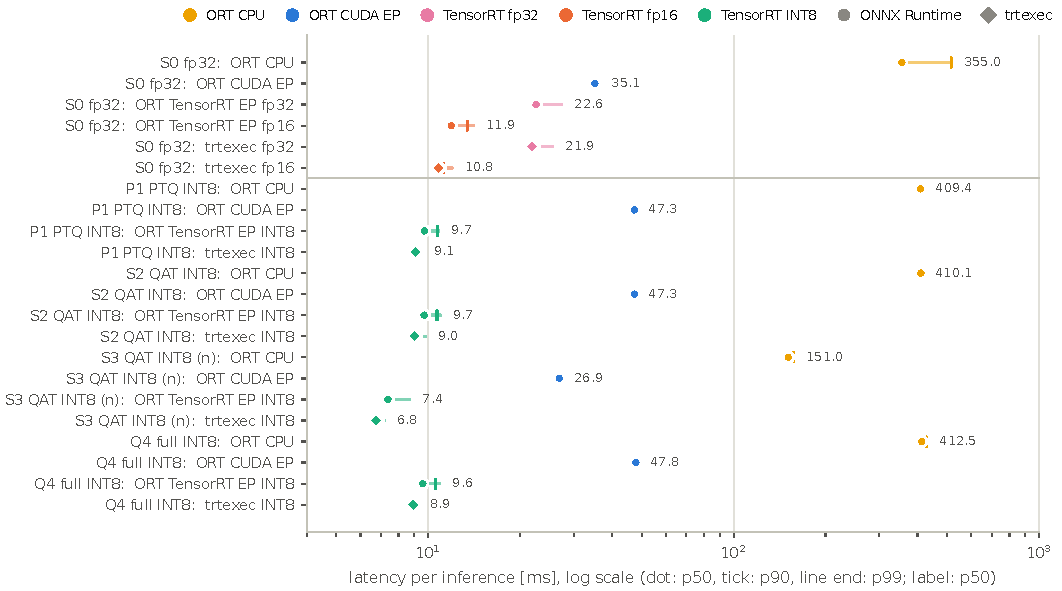
\includegraphics[width=\textwidth]{bench_latency.pdf}
\caption{Inference latency per model and backend (log scale). Dot: median; tick: p90; end of the line: p99. Colour:
backend family; shape: ONNX Runtime or \codeb{trtexec}.}\label{fig:bench_latency}
\end{figure}

\begin{figure}[t]
\centering
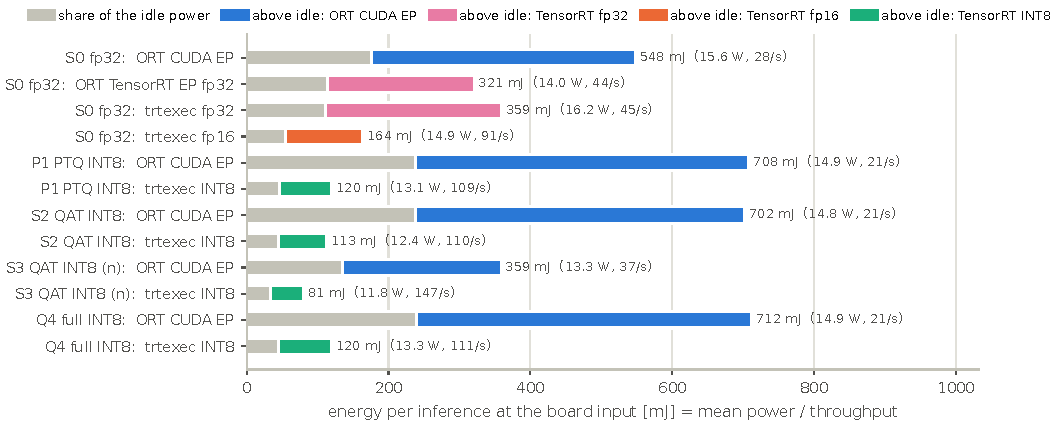
\includegraphics[width=\textwidth]{bench_energy.pdf}
\caption{Energy per inference at the board input for the validated measurement windows. The grey part is the share of
the idle power ($P_{\mathrm{idle}}/r$); the coloured part is the energy above idle.}\label{fig:bench_energy}
\end{figure}

\begin{table}[t]
\centering\footnotesize
\caption{Inference benchmark. $\bar P$: mean board input power in the measurement loop; GPU: mean GPU load in the same
window; $E_{\mathrm{inf}}$, $E_{\mathrm{dyn}}$: energy per inference, total and above idle. Missing values: windows
rejected by the validity rule of \cref{sec:stats}.}\label{tab:bench}
\begin{tabular}{@{}llrrrrrrr@{}}
\toprule
Model & Backend & p50 & p99 & Rate & $\bar P$ & GPU & $E_{\mathrm{inf}}$ & $E_{\mathrm{dyn}}$ \\
 & & [ms] & [ms] & [1/s] & [W] & [\%] & [mJ] & [mJ] \\
\midrule
S0 fp32 & ORT CPU & 354.99 & 515.09 & 2.5 & 8.54 & 0 & 3416 & 1409 \\
 & ORT CUDA EP & 35.08 & 36.14 & 28.5 & 15.62 & 95 & 548 & 372 \\
 & ORT TensorRT EP fp32 & 22.55 & 27.35 & 43.8 & 14.05 & 59 & 321 & 206 \\
 & ORT TensorRT EP fp16 & 11.91 & 14.07 & 82.1 & -- & 23 & -- & -- \\
 & trtexec fp32 & 21.87 & 25.55 & 45.2 & 16.22 & 83 & 359 & 248 \\
 & trtexec fp16 & 10.81 & 11.96 & 90.9 & 14.89 & 71 & 164 & 109 \\
\addlinespace
P1 PTQ INT8 & ORT CPU & 409.39 & 415.86 & 2.4 & 8.60 & 0 & 3583 & 1493 \\
 & ORT CUDA EP & 47.29 & 47.83 & 21.1 & 14.95 & 91 & 708 & 471 \\
 & ORT TensorRT EP INT8 & 9.71 & 10.80 & 101.6 & -- & 0 & -- & -- \\
 & trtexec INT8 & 9.10 & 9.49 & 109.1 & 13.10 & 71 & 120 & 74 \\
\addlinespace
S2 QAT INT8 & ORT CPU & 410.06 & 415.32 & 2.4 & 8.73 & 0 & 3636 & 1545 \\
 & ORT CUDA EP & 47.34 & 47.83 & 21.1 & 14.82 & 90 & 702 & 465 \\
 & ORT TensorRT EP INT8 & 9.70 & 10.96 & 101.5 & -- & 0 & -- & -- \\
 & trtexec INT8 & 9.02 & 9.78 & 110.2 & 12.44 & 56 & 113 & 67 \\
\addlinespace
S3 QAT INT8 (n) & ORT CPU & 151.04 & 156.99 & 6.6 & -- & 0 & -- & -- \\
 & ORT CUDA EP & 26.88 & 27.32 & 37.2 & 13.34 & 83 & 359 & 224 \\
 & ORT TensorRT EP INT8 & 7.38 & 8.69 & 134.3 & -- & 0 & -- & -- \\
 & trtexec INT8 & 6.75 & 7.18 & 146.6 & 11.81 & 72 & 81 & 46 \\
\addlinespace
Q4 full INT8 & ORT CPU & 412.46 & 428.20 & 2.4 & 8.70 & 0 & 3623 & 1533 \\
 & ORT CUDA EP & 47.83 & 48.38 & 20.9 & 14.88 & 94 & 712 & 472 \\
 & ORT TensorRT EP INT8 & 9.59 & 10.90 & 102.4 & -- & 0 & -- & -- \\
 & trtexec INT8 & 8.92 & 9.19 & 111.4 & 13.31 & 70 & 120 & 75 \\
\bottomrule
\end{tabular}

\end{table}

\subsection{The detector node (RQ2)}\label{sec:detector}
\Cref{tab:detector,tab:comparisons,fig:detector_ecdf,fig:detector_resources} summarize the detector runs.

\textbf{Backend.} In the node, the median inference time is 46.43\,ms with ONNX Runtime's CUDA EP, 17.15\,ms with the
TensorRT fp16 engine and 15.10\,ms with the INT8 engine (Jazzy, native). TensorRT reduces it to 0.369 of the ONNX
Runtime value, 95\,\% CI [0.369, 0.370]. The distributions do not overlap at all (Cliff's $\delta = -1$). The node
adds about 6\,ms to the engine's own latency with TensorRT (17.15 vs.\ 10.81\,ms; INT8: 15.10 vs.\ 9.02\,ms) and
11\,ms with ONNX Runtime (46.43 vs.\ 35.08\,ms). \Cref{sec:gpu} traces this overhead to preprocessing on the CPU and
the upload of a float32 tensor. TensorRT also changes the node's footprint: 0.53 instead of 1.44\,GB of resident
memory ($-0.91$\,GB), 5--8 instead of 15--19\,\% GPU load, and 5.85 instead of 6.97\,W ($-1.1$\,W). Since the node
works at a fixed 5\,Hz (measured: 5.00\,Hz, inter-arrival standard deviation 0.3--0.6\,ms), the energy per
detection falls from 1.39 to 1.17\,J at the board input. Above idle it falls from 0.39 to 0.17\,J.

\textbf{Cold start.} The first inference takes 1.50--1.62\,s with the CUDA EP, which selects and loads its kernels
lazily, but only 34--87\,ms with a deserialized TensorRT engine.

\textbf{Distribution.} Between Jazzy and Kilted, the median changes by $-0.10$\,ms (TensorRT, $\delta = -0.37$) and
$+0.07$\,ms (ONNX Runtime, $\delta = +0.23$). Both differences are statistically detectable but below 1\,\% and
practically irrelevant. Under Lyrical (Isaac Buildfarm, native) the node's memory, CPU and power match the other
distributions (\cref{fig:detector_resources}). Its inference times were not recorded, because bag recording failed
with the Lyrical runtimes at the time (fixed since, \finding{68}). Two 25-second verification runs after the fix, outside
the campaign, give medians of 17.27\,ms for Lyrical on Ubuntu 24.04 and 19.43\,ms for Lyrical on Ubuntu 26.04 in its
container; the latter difference would need replicates before it can be interpreted.

\textbf{Run-time mode and replicate.} In the container, the median is 0.55\,ms higher than natively (95\,\% CI
[0.50, 0.59], $\delta = +0.94$). A second native run under identical conditions, however, differs from the first by
$+0.48$\,ms ($\delta = +0.92$), and its resident memory (0.68\,GB) equals the container's
(\cref{fig:detector_ecdf}b). The container effect is therefore not separable from run-to-run variation. Within this
design, the container costs at most about 0.6\,ms (3\,\%) and no measurable memory. The comparison is also confounded
by the DDS implementation (Cyclone DDS in the container, Fast DDS natively).

\begin{keybox}[Revision of an earlier conclusion]
The system documentation (\code{jxb.pdf}, based on single runs) reported a container overhead of $+0.6$\,ms and
$+155$\,MB. The replicate shows that both differences are within the run-to-run variation of the native
configuration.
\end{keybox}

\begin{table}[t]
\centering\footnotesize
\caption{The detector node with the synthetic camera. Median with 95\,\% block-bootstrap interval; Det.\ CPU/RSS:
the detector process; GPU and $\bar P$: board means; $E_{\mathrm{det}}$: board energy per detection. Runs marked --
have no per-frame inference data.}\label{tab:detector}
\setlength{\tabcolsep}{4pt}
\begin{tabular}{@{}lrrrrrrrrr@{}}
\toprule
Configuration & $n$ & Median [ms] & p99 & Rate & Det.\ CPU & Det.\ RSS & GPU & $\bar P$ & $E_{\mathrm{det}}$ \\
 & & (95\,\% CI) & [ms] & [Hz] & [cores] & [GB] & [\%] & [W] & [J] \\
\midrule
Jazzy ORT CUDA EP & 199 & 46.43 (46.40--46.46) & 46.9 & 5.00 & 0.17 & 1.44 & 15.4 & 6.97 & 1.39 \\
Jazzy ORT CUDA EP (rep.) & -- & -- & -- & -- & 0.19 & 1.43 & 19.3 & 7.00 & -- \\
Jazzy TRT fp16 & 207 & 17.15 (17.14--17.17) & 18.3 & 5.00 & 0.11 & 0.53 & 5.1 & 5.85 & 1.17 \\
Jazzy TRT INT8 (QAT) & 206 & 15.10 (15.08--15.12) & 16.3 & 5.00 & 0.12 & 0.52 & 5.5 & 5.67 & 1.13 \\
Kilted ORT CUDA EP & 202 & 46.50 (46.47--46.54) & 46.9 & 5.00 & 0.23 & 1.44 & 16.4 & 7.07 & 1.41 \\
Kilted TRT fp16 & 210 & 17.05 (17.02--17.09) & 17.5 & 5.00 & 0.14 & 0.54 & 7.3 & 5.91 & 1.18 \\
Kilted TRT fp16 (rep.) & 131 & 17.53 (17.50--17.55) & 18.3 & 5.00 & 0.13 & 0.68 & 6.6 & 5.90 & 1.18 \\
Kilted TRT fp16, container & 205 & 17.60 (17.57--17.63) & 18.3 & 5.00 & 0.15 & 0.68 & 8.1 & 5.97 & 1.19 \\
Lyrical ORT CUDA EP & -- & -- & -- & -- & 0.21 & 1.55 & 18.5 & 6.99 & -- \\
Lyrical TRT fp16 & -- & -- & -- & -- & 0.13 & 0.63 & 5.8 & 5.89 & -- \\
Lyrical 26.04 TRT fp16, container & -- & -- & -- & -- & 0.17 & 0.68 & 5.0 & 5.92 & -- \\
\bottomrule
\end{tabular}

\end{table}

\begin{table}[t]
\centering\footnotesize
\caption{Pairwise comparisons of the detector's inference time: median difference with 95\,\% block-bootstrap
interval, ratio of medians, Cliff's $\delta$ (positive: $y$ slower).}\label{tab:comparisons}
\setlength{\tabcolsep}{4pt}
\begin{tabular}{@{}llrrrr@{}}
\toprule
Factor & Comparison ($x \to y$) & $\tilde y - \tilde x$ [ms] (95\,\% CI) & $\tilde y / \tilde x$ & Cliff's $\delta$ & $n_x / n_y$ \\
\midrule
backend & ORT CUDA EP $\to$ TensorRT fp16 (Jazzy) & -29.28 (-29.31 to -29.25) & 0.369 & -1.00 & 199/207 \\
backend & TensorRT fp16 $\to$ INT8 (Jazzy) & -2.05 (-2.08 to -2.02) & 0.881 & -1.00 & 207/206 \\
distro & Jazzy $\to$ Kilted (TensorRT fp16) & -0.10 (-0.14 to -0.06) & 0.994 & -0.37 & 207/210 \\
distro & Jazzy $\to$ Kilted (ORT CUDA EP) & +0.07 (+0.03 to +0.11) & 1.001 & +0.23 & 199/202 \\
mode & native $\to$ container (Kilted, TensorRT fp16) & +0.55 (+0.50 to +0.59) & 1.032 & +0.94 & 210/205 \\
replicate & run $\to$ replicate (Kilted TensorRT fp16) & +0.48 (+0.42 to +0.51) & 1.028 & +0.92 & 210/131 \\
load & alone $\to$ in the stack (TensorRT fp16) & +8.07 (+7.59 to +8.46) & 1.473 & +1.00 & 210/569 \\
load & alone $\to$ in the stack (ORT CUDA EP) & +13.71 (+13.18 to +14.23) & 1.295 & +1.00 & 202/559 \\
\bottomrule
\end{tabular}

\end{table}

\begin{figure}[t]
\centering
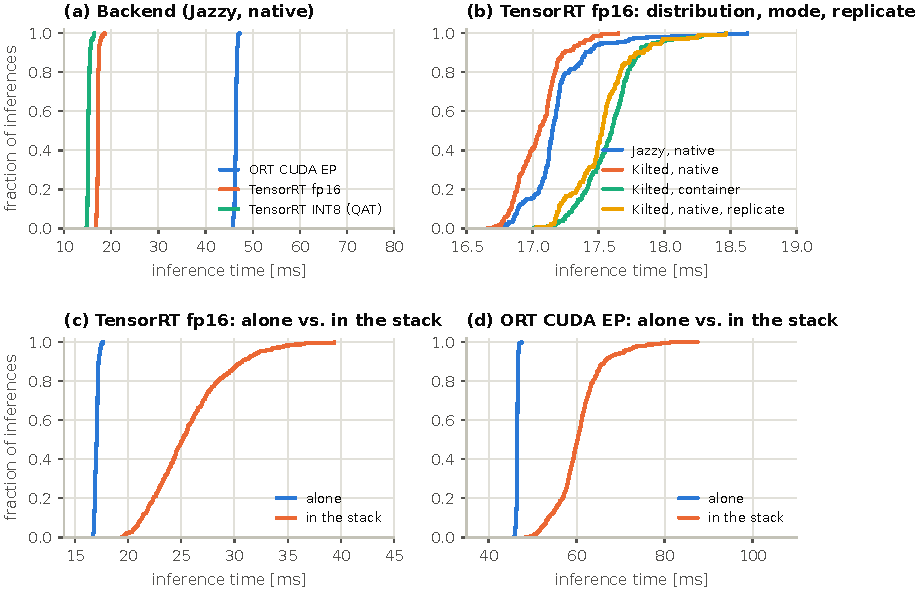
\includegraphics[width=\textwidth]{detector_ecdf.pdf}
\caption{Empirical distribution functions of the detector's per-frame inference time. (a) Backends; (b) TensorRT fp16
across distributions, run-time modes and a replicate; (c, d) the node alone and inside the full stack.}
\label{fig:detector_ecdf}
\end{figure}

\begin{figure}[t]
\centering
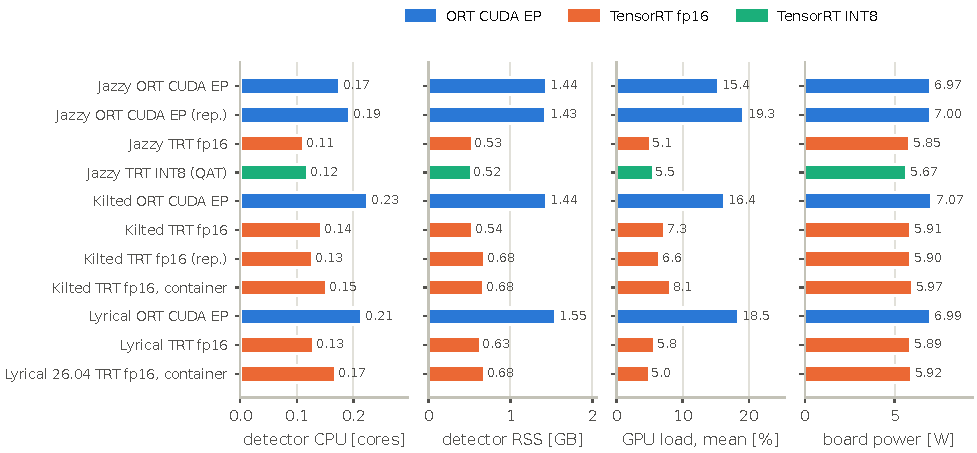
\includegraphics[width=\textwidth]{detector_resources.pdf}
\caption{Resources of the detector node per configuration: CPU and resident memory of the detector process, mean GPU
load and board power.}\label{fig:detector_resources}
\end{figure}

\subsection{The full stack (RQ3)}\label{sec:stack}
\Cref{tab:stack,fig:stack_breakdown,fig:stack_timeseries} characterize the full stack. In every configuration, all
processes started and stopped cleanly.

\textbf{Load.} With the TensorRT fp16 detector, the stack runs at 2.83 CPU cores (60\,\% mean load of the six cores),
2.11\,GB summed peak resident memory, 13.8\,\% mean GPU load and 8.54\,W, which is 3.52\,W above idle. The maximum
junction temperature is 53.0\,\si{\celsius}. The composable-node container of the image pipeline dominates with 1.64
cores, 58\,\% of the session's CPU. It is followed by the measurement and launch tools (0.39 cores), the synthetic
camera (0.36), the detector (0.33) and ten other nodes (0.11 together). With ONNX Runtime instead of TensorRT, the
stack needs 0.10 cores and 0.81\,GB more and draws 1.16\,W more, and its GPU load doubles to 29.7\,\%. In the
container the stack is indistinguishable from native execution within single runs: 2.75 cores, 2.07\,GB, 8.51\,W.

\textbf{Composition.} With one process per node, the session needs 2.36 cores. This configuration ran without bag
recorder and rate probes, however: its tools use 0.02 cores instead of 0.39. The image pipeline's own CPU is the
same in both arrangements (1.57 vs.\ 1.64 cores), while its seven separate processes hold 0.74 instead of 0.52\,GB.
Composition thus saves memory, partly by sharing library pages, but no measurable CPU. This suggests that
intra-process communication does not take effect in the composed container (\hyp{2}).

\textbf{Throughput.} The camera delivers 30 frames per second, but lane points are produced at 23.3\,Hz, and the
Nsight Systems trace (without rate probes) shows the image pipeline processing 24.2 frames per second. A fifth of the
frames is lost before the lane detection. The rate probe on the undistorted image topic (\code{ros2 topic hz}) reports
only 19.8--20.5\,Hz (\cref{fig:stack_rates}). It has to receive every $1280\times800$ image (3\,MB) in a separate
process, and on the loaded board it under-reports the rate. Detections arrive at the node's 5\,Hz.

\textbf{Detector under load.} Inside the stack, the detector's median inference time rises from 17.05 to 25.12\,ms
($\times 1.47$, CI of the difference [7.59, 8.46]\,ms) and its p99 to 36.3\,ms. With ONNX Runtime it rises from 46.50 to
60.21\,ms ($\times 1.30$).

\textbf{Power.} \Cref{fig:power_rails} decomposes the board power. From idle to the full stack, the CPU/GPU/CV rail
grows from 1.10 to 3.25\,W (+2.15\,W). This is the largest increase, consistent with a CPU-heavy workload. The rest of
the module grows by 0.92\,W, which we attribute mainly to memory traffic, and the SoC rail by 0.45\,W.

\textbf{Memory growth.} In every stack configuration, the system's used memory grows linearly while the stack runs:
+284\,MB/min natively, +255\,MB/min in the container, +215\,MB/min with ONNX Runtime and +213\,MB/min per node,
without bag recorder and probes (\cref{fig:stack_memory}). The summed resident memory of the session's processes stays
flat ($-4$ to $+11$\,MB/min). The growth is therefore not process memory, and the bag recorder does not cause it. If
it continued linearly, the remaining 4.5\,GB would be exhausted within another 16--21 minutes. The follow-up run of
\cref{sec:memtest} shows that it does not continue (\hyp{7}).

\begin{table}[t]
\centering\footnotesize
\caption{The full stack (120\,s each, Kilted). CPU: session share in cores; RSS: summed peak resident memory; GPU,
$\bar P$: means after the start-up phase; $P_{\mathrm{dyn}} = \bar P - P_{\mathrm{idle}}$; Lanes: lane-point rate
(bag); Undist.: median of the rate probe on undistorted images; RAM slope: growth of the system's used memory.
*: one process per node, without bag recorder and rate probes.}\label{tab:stack}
\setlength{\tabcolsep}{3.5pt}
\begin{tabular}{@{}lrrrrrrrrr@{}}
\toprule
Configuration & CPU & RSS & GPU & $\bar P$ & $P_{\mathrm{dyn}}$ & Lanes & Undist. & Inference & RAM slope \\
 & [cores] & [GB] & [\%] & [W] & [W] & [Hz] & [Hz] & p50/p99 [ms] & [MB/min] \\
\midrule
ORT CUDA EP, native & 2.93 & 2.92 & 29.7 & 9.70 & 4.68 & 23.2 & 19.8 & 60.2 / 78.0 & 215 \\
TRT fp16, native & 2.83 & 2.11 & 13.8 & 8.54 & 3.52 & 23.3 & 20.0 & 25.1 / 36.3 & 284 \\
TRT fp16, container & 2.75 & 2.07 & 14.0 & 8.51 & 3.50 & 23.3 & 20.5 & 25.3 / 39.9 & 255 \\
TRT fp16, native, per node* & 2.36 & 1.92 & 14.3 & 8.25 & 3.24 & -- & -- & -- & 213 \\
\bottomrule
\end{tabular}

\end{table}

\begin{figure}[t]
\centering
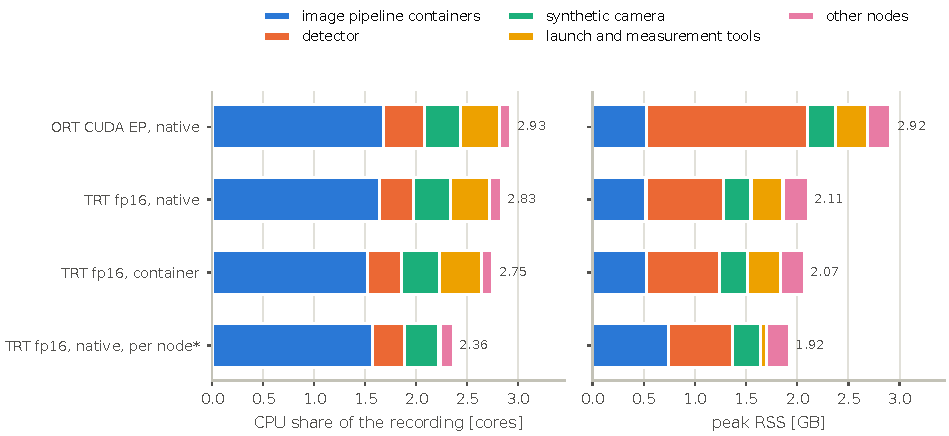
\includegraphics[width=\textwidth]{stack_breakdown.pdf}
\caption{CPU share and peak resident memory of the stack by process category.}\label{fig:stack_breakdown}
\end{figure}

\begin{figure}[p]
\centering
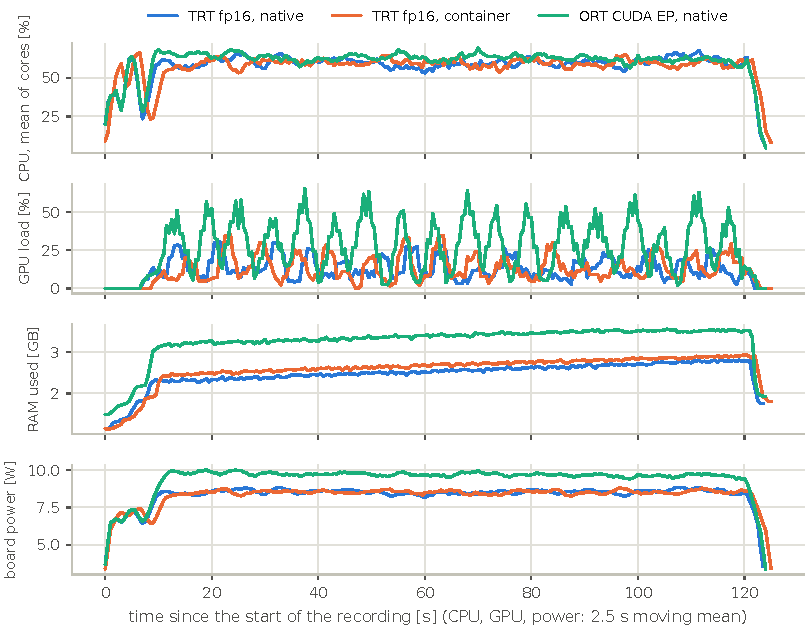
\includegraphics[width=\textwidth]{stack_timeseries.pdf}
\caption{Board telemetry of three stack runs over time: mean CPU load, GPU load, used memory and board power. The GPU
load shows periodic bursts with a period of about 6--7\,s; the data does not reveal their cause (the synthetic scene
repeats every 2\,s).}\label{fig:stack_timeseries}
\end{figure}

\begin{figure}[t]
\centering
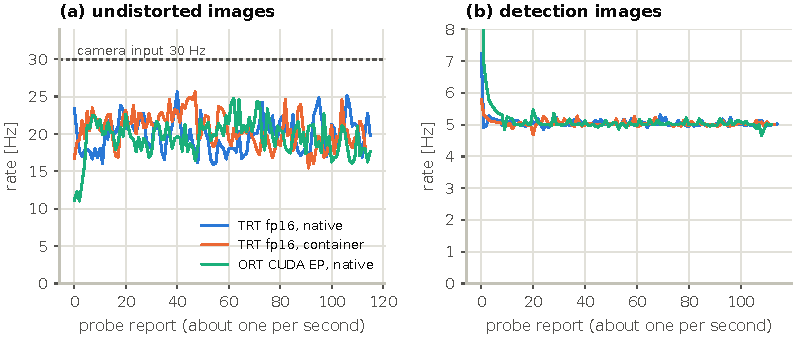
\includegraphics[width=\textwidth]{stack_rates.pdf}
\caption{Rates reported by the rate probes about once per second: (a) undistorted images, (b) detection images.}
\label{fig:stack_rates}
\end{figure}

\begin{figure}[t]
\centering
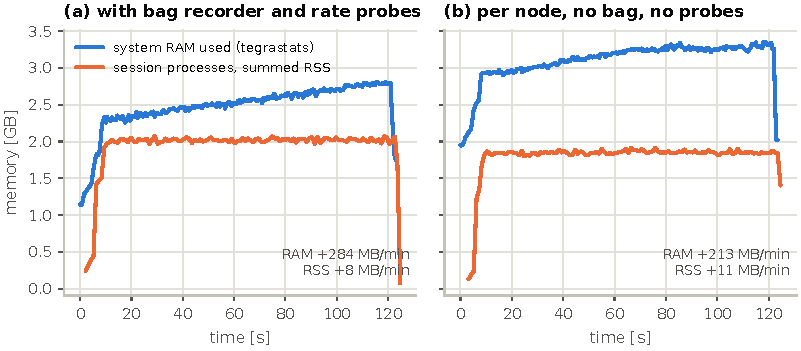
\includegraphics[width=\textwidth]{stack_memory.pdf}
\caption{Used system memory (tegrastats) and summed resident memory of the session's processes during two stack runs,
with linear slopes over the steady phase.}\label{fig:stack_memory}
\end{figure}

\begin{figure}[t]
\centering
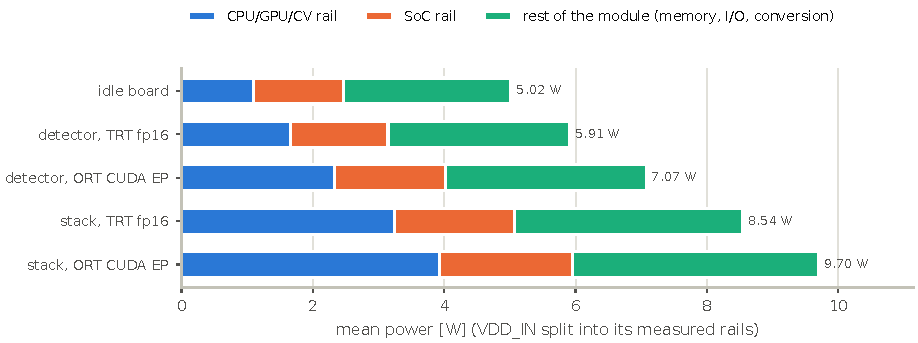
\includegraphics[width=\textwidth]{power_rails.pdf}
\caption{Mean board input power split into the measured rails, from the idle board to the full stack.}
\label{fig:power_rails}
\end{figure}

\subsection{Long-duration memory behaviour (follow-up)}\label{sec:memtest}
To decide \hyp{7}, the stack was run for 25 minutes on 2026-11-04 in its TensorRT configuration (Kilted, native,
INFO logging as before), without bag recorder and rate probes. Next to the per-process sampler, \jxb{} recorded the
kernel's memory counters (\code{/proc/meminfo}) every second. A memory guard would have stopped the launch below
1.2\,GB of available memory; it did not fire. All 12 processes ran and stopped cleanly; the session used 2.60 cores,
1.85\,GB summed peak resident memory and 8.33\,W, and the junction temperature stayed below 55\,\si{\celsius}.

The used memory rises steeply during the first two minutes (+322\,MB/min) and slower until the third (+34\,MB/min),
and then stays at 2.99\,GB (3057\,MB), against 1.17\,GB before the start (\cref{fig:memtest}). From minute 10 on it grows by
only 3\,MB/min, and the page cache grows by 5\,MB/min, as the ROS log files grow. \code{Shmem} (5\,MB), \code{Slab}
and unreclaimable kernel memory stay constant; \code{MemAvailable} settles at 4.27\,GB. The recordings of
\cref{sec:stack}, two minutes long, captured only this warm-up. The session's resident memory reaches its level within
10\,s, so the slower ramp of the used memory is memory outside the processes' resident sets that is allocated while the
pipeline warms up. Device memory allocated through the CUDA driver, such as stream-ordered memory pools, is an
explanation consistent with this; the counters available without root cannot attribute it further.

\begin{figure}[t]
\centering
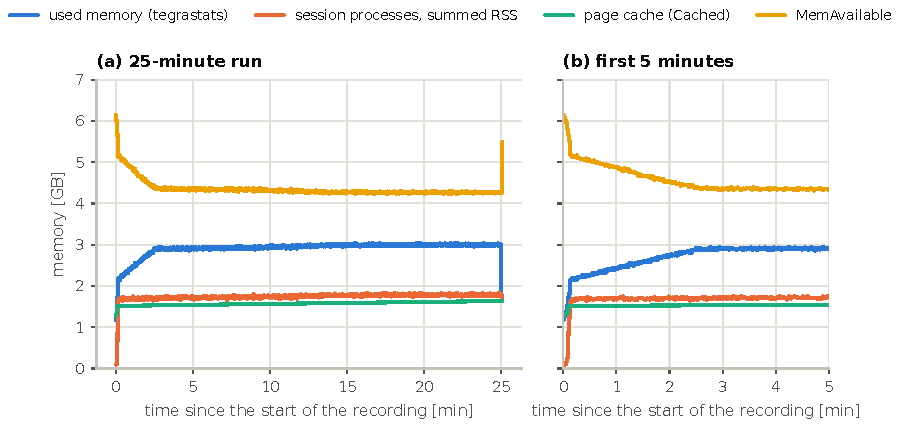
\includegraphics[width=\textwidth]{memtest.pdf}
\caption{The 25-minute follow-up run: used memory, summed resident memory of the session, page cache and available
memory. The growth seen in the two-minute recordings is a warm-up of about three minutes.}\label{fig:memtest}
\end{figure}

\subsection{Anomalies}\label{sec:anomalies}
\textbf{The reset.} The board reset about 4\,s into a run of the detector with ONNX Runtime's CUDA EP inside the Kilted
runtime container, while the EP was initializing (\finding{56}). \Cref{tab:reset} shows the last telemetry before the
reset: memory rising from 1.39 to 1.50\,GB as the model loads, CPU load up to 44\,\%, GPU idle, at most 6.7\,W and
49--50\,\si{\celsius}. At this resolution no thermal or power anomaly precedes the reset. The kernel's panic log, read
later from pstore with root, explains it (\finding{79}): an Oops in \code{kswapd0}, during page reclaim, where freeing
buffer heads charged to a memory cgroup dereferenced an invalid address (\code{obj_cgroup_uncharge} $\to$
\code{refill_obj_stock}) on the PREEMPT\_RT kernel, followed by a kernel panic. It was a kernel bug; the CUDA EP's
initialization in the container only supplied the memory pressure.

\textbf{Long nsys sessions.} In two Nsight Systems recordings, the session stayed open long after the workload had
ended (508\,s and 3800\,s). Nsight Systems waits for every process of the profiled tree, including processes that
survive the workload. The first case is the launch that died at start (\finding{62}). For these recordings, telemetry
means would be dominated by the idle tail; we restrict the analysis to the GPU-active window. The tail of the second
recording provides the idle baseline.

% ===================================================================================================== 4
\section{GPU-level analysis}\label{sec:gpu}
The Nsight Systems trace of the full stack (TensorRT fp16, without rate probes) explains the throughput limit. Its
GPU-active window lasts 25.9\,s and contains 29\,440 kernels; the GPU is busy 11.1\,\% of the window.
\Cref{fig:nsys,fig:gpu_timeline,tab:per_frame} summarize it.

\textbf{The image pipeline is not GPU-bound.} It launches seven kernels per frame (image warp 0.95\,ms, remap
0.49\,ms, a vertical mean-and-threshold step 0.27\,ms, \dots), 2.17\,ms of GPU time per frame. At that cost the GPU
could serve more than 400 frames per second. Instead, each frame costs 14.6\,ms of blocking CUDA API time in 36.5
calls. Of these, 16 calls (9.1\,ms) allocate or free device memory: seven pairs of \code{cudaMalloc}/\code{cudaFree}
and one pair of \code{cudaMallocAsync}/\code{cudaFreeAsync} per frame. \code{cudaFree} implicitly synchronizes the
device, so these calls also serialize the pipeline. Allocations and frees are balanced in both GPU processes
(\code{cudaMalloc} 4394, \code{cudaFree} 4397; async 627/627), so the trace shows no device memory leak. Per frame, the
pipeline uploads 3.09\,MB (one RGB frame) and downloads 4.94\,MB (1.6 frames). On a SoC whose CPU and GPU share the
same DRAM, these copies move data within the same physical memory. \code{memcpy} is the hottest CPU function of the
image pipeline (12.4\,\% of its CPU samples), followed by atomic exchange and compare-and-swap primitives, which
indicate lock traffic.

\textbf{The detector's slowdown is not GPU contention.} In the stack, an inference takes 196 kernels and 12.2\,ms of
GPU time, 16\,\% more than the engine's 10.5\,ms GPU compute time in isolation. The detector's kernels overlap with
those of the image pipeline for only 44\,ms of their 1560\,ms (2.8\,\%), however. Most of the 8\,ms increase of
the inference time must therefore arise outside the GPU kernels. Candidates are CPU-side pre- and postprocessing
on a busy CPU, waits, and memory bandwidth. The detector's CPU profile supports this: besides \code{memcpy}, OpenCV's
float32 channel split and subtraction (\code{cv::hal::split32s}, \code{cv::hal::sub32f}) appear among its hottest
functions. The node prepares the normalized float32 input on the CPU and uploads it: 7.2\,MB per inference, the size
of a $1\times3\times608\times960$ float32 tensor.

\textbf{ONNX Runtime's CUDA EP.} In the isolated benchmark, the GPU is busy only 52.6\,\% of the CUDA EP's active
window, against 78.4\,\% with the TensorRT EP. \code{cudaMemcpyAsync} takes 962\,ms of API time for 672 calls, while the
copy engine needs 55\,ms for the 430\,MB involved: the inputs come from pageable host memory and are staged
synchronously. Layout conversions (\code{nchwToNhwcKernel}) take 6.4\,\% of the GPU time.

\begin{figure}[t]
\centering
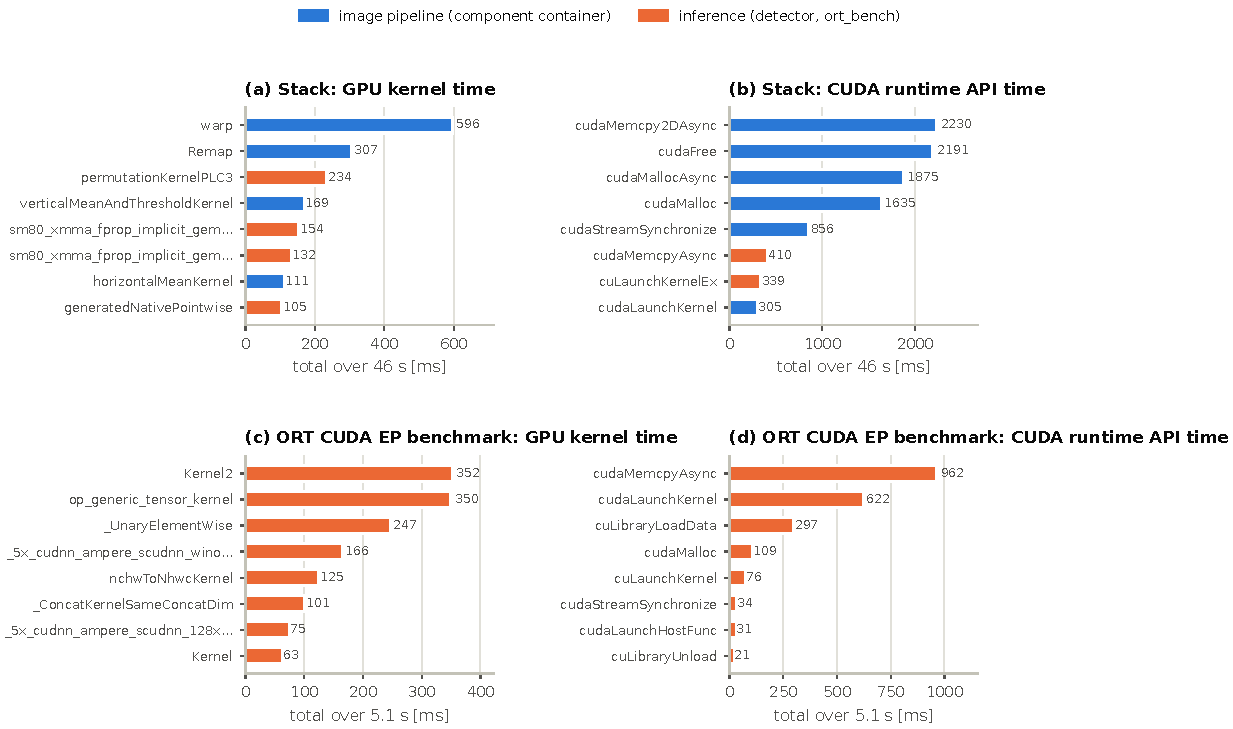
\includegraphics[width=\textwidth]{nsys_breakdown.pdf}
\caption{Nsight Systems: top kernels and CUDA runtime API calls by total time in the stack trace (a, b) and in the ONNX
Runtime CUDA EP benchmark (c, d). Colour: process role.}\label{fig:nsys}
\end{figure}

\begin{figure}[t]
\centering
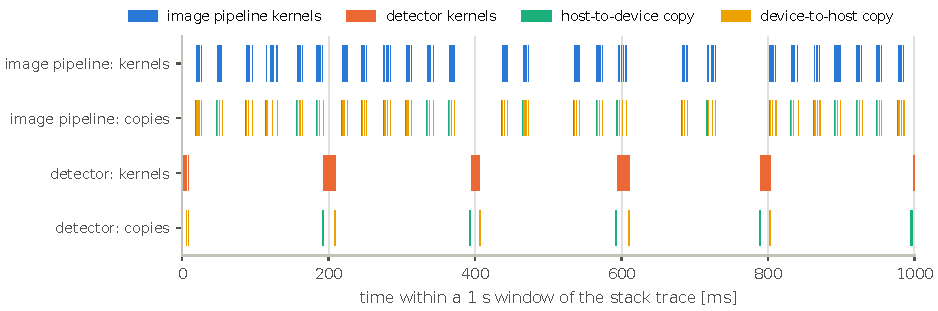
\includegraphics[width=\textwidth]{gpu_timeline.pdf}
\caption{One second of GPU activity in the stack: the image pipeline's per-frame kernel bursts with their copies, and
the detector's 5\,Hz inferences. The GPU is idle most of the time; gaps in the image pipeline's rhythm are frames it
did not process.}\label{fig:gpu_timeline}
\end{figure}

\begin{table}[t]
\centering\small
\caption{Cost of one processed frame in the image pipeline (Nsight Systems, full stack, TensorRT fp16).}
\label{tab:per_frame}
\begin{tabular}{@{}lr@{}}
\toprule
Quantity (image pipeline, per processed frame) & Value \\
\midrule
processed frames in the GPU-active window & 627 (24.2 Hz) \\
GPU kernel time & 2.17 ms \\
CUDA runtime API time (blocking, summed over threads) & 14.62 ms \\
CUDA runtime API calls & 36.5 \\
device allocations and frees (\texttt{cudaMalloc}, \texttt{cudaFree}, async variants) & 16.0 calls, 9.11 ms \\
host-to-device copies & 3.09 MB \\
device-to-host copies & 4.94 MB \\
copy engine time & 1.08 ms \\
share of CPU samples in \texttt{memcpy} (leaf) & 12.4\,\% \\
\bottomrule
\end{tabular}

\end{table}

% ===================================================================================================== 5
\section{Discussion}\label{sec:discussion}

\subsection{Answers to the research questions}
\textbf{RQ1.} TensorRT engines are the most efficient backend by a wide margin, in latency (3.2$\times$ against the
CUDA EP) and in energy (3.3$\times$). INT8 adds 16--18\,\% for the s-sized model; the n-sized INT8 model is the
fastest option at 6.75\,ms. ONNX Runtime's TensorRT EP retains most of the benefit (+10\,\% latency) while keeping the
ONNX Runtime API. Quantized models must not run without TensorRT.

\textbf{RQ2.} Neither the ROS~2 distribution nor the run-time mode has a practically relevant effect on the
detector: distribution effects stay below 1\,\%, and the container effect (+0.55\,ms) is as large as the variation
between two native runs (+0.48\,ms). The choice between native and container execution, and between Jazzy, Kilted and
Lyrical, can therefore be made on functional grounds.

\textbf{RQ3.} The full stack uses less than half of the board's CPU capacity, an eighth of its GPU and a third of its
25\,W budget, yet it does not keep up with the camera. The bottleneck is the image pipeline's data handling: device
memory allocated and freed several times per frame, frames copied between host and device memory although both are
the same DRAM, CPU-side copies and lock traffic. The arithmetic itself costs little. The detector's slowdown in the
stack has the same root: it competes for CPU and memory, not for the GPU.

\subsection{A frame-cost model}
At 30\,Hz, a frame must pass the pipeline every 33.3\,ms. The image pipeline spends 2.2\,ms of GPU time per frame but
14.6\,ms in blocking CUDA calls and, measured by its CPU share, $1.64 / 24.2\,\mathrm{Hz} = 68$\,ms of CPU time per
frame across its threads. If the per-frame API time lies on the critical path, it alone takes 44\,\% of the frame
budget. Removing the allocation calls (9.1\,ms) would shorten that path by more than the remaining margin to 30\,Hz.
This is the quantitative basis of \hyp{1}.

\subsection{The observer effect}
The measurement tools are not free. The bag recorder and the two Python rate probes use 0.37 cores, 13\,\% of the
session's CPU. The probes also add DDS subscribers to large image topics, which costs the publishers copies. The probe
on the undistorted images even underestimates the rate it measures. Lightweight probes are therefore a prerequisite
for precise A/B experiments on the stack (\hyp{8}). The 1\,s per-process sampler costs 0.9--1.1\,\% of one core.

% ===================================================================================================== 6
\section{Optimization hypotheses (RQ4)}\label{sec:hypotheses}
Each hypothesis states the observation it rests on, the mechanism, a quantified prediction and an experiment that can
falsify it with \jxb{}. \Cref{tab:hyp} ranks them by expected benefit and effort.

\begin{hypbox}{H1: Reusing device buffers in the image pipeline raises its frame rate}
\textbf{Observation.} 16 allocation and free calls per frame, 9.1\,ms of blocking API time; \code{cudaFree}
synchronizes the device (\cref{tab:per_frame}). A kernel trace of the stack shows the cost on the kernel side too:
nvmap's page-zeroing thread \code{nvmap-bz} takes 0.39 cores (\finding{80}).
\par\textbf{Mechanism.} Frame-sized buffers are allocated per frame. Preallocating them once (buffer pool, CV-CUDA tensor
reuse) or using the stream-ordered allocator with a memory-pool release threshold removes the calls and the implicit
synchronization.
\par\textbf{Prediction.} The allocation calls per frame drop from 16 to about 0; the image pipeline reaches at least
28\,Hz with the 30\,Hz camera (lane points $\ge 28$\,Hz); its CPU share falls by 10--25\,\%, and up to 0.4 cores of
kernel page zeroing disappear.
\par\textbf{Test.} Patch the image processing component; record \code{jxb trace nsys} (allocations per frame) and
\code{jxb launch --monitor --bag} (lane-point rate, CPU) before and after, three runs each.
\end{hypbox}

\begin{hypbox}{H2: A GPU-resident data path removes most copies and CPU memcpy}
\textbf{Observation.} Per frame 3.1\,MB host-to-device and 4.9\,MB device-to-host; \code{memcpy} is the image pipeline's
hottest CPU function (12.4\,\%); composition saves no CPU against separate processes.
\par\textbf{Mechanism.} CPU and GPU share the DRAM, so frames can stay in device-accessible memory (pinned and mapped
host memory, or unified memory, see the CUDA for Tegra notes~\cite{cuda-tegra}). Between composed nodes they can be
passed without serialization through intra-process communication with type adaptation (REP~2007~\cite{rep2007}) or
Lyrical's \code{rosidl::Buffer} CUDA backend.
\par\textbf{Prediction.} Copy volume per frame below 1\,MB; \code{memcpy} below 3\,\% of the image pipeline's samples;
image pipeline CPU $-20$\,\%; \enquote{rest of the module} power $-0.2$ to $-0.4$\,W.
\par\textbf{Test.} \code{jxb trace nsys} (copy volume, CPU samples) and \code{--monitor} (CPU, rails) before and after.
\end{hypbox}

\begin{hypbox}{H3: Preprocessing on the GPU shortens the detector's node overhead}
\textbf{Observation.} About 6\,ms between engine latency and node inference time (TensorRT); 7.2\,MB float32 upload per
inference; OpenCV float32 split and subtract among the detector's hottest functions.
\par\textbf{Mechanism.} Upload the 8-bit image (1.75\,MB at $960\times608$) and convert, normalize and transpose it on the
GPU (CV-CUDA or a preprocessing layer in the engine). Models with 8-bit NHWC input, such as SAM's newer YOLO26
models (\finding{55}), make this the default.
\par\textbf{Prediction.} Node overhead from 6 to 2--3\,ms alone (inference time about 13--14\,ms with fp16); a larger gain in
the stack, where the CPU is contended (25.1\,ms $\to$ below 20\,ms); detector CPU $-0.05$ to $-0.1$ cores.
\par\textbf{Test.} Bag inference time alone and in the stack; host-to-device volume per inference in nsys.
\end{hypbox}

\begin{hypbox}{H4: Scheduling priorities contain the detector's slowdown in the stack}
\textbf{Observation.} +8.1\,ms median and p99 of 36\,ms in the stack, with 2.8\,\% kernel overlap.
\par\textbf{Mechanism.} The detector's CPU threads compete with the image pipeline on a PREEMPT\_RT kernel. Real-time
priorities (\code{SCHED_FIFO}) and CPU affinity for the detector, and a high-priority CUDA stream for its inference,
shorten its waits.
\par\textbf{Prediction.} In-stack median below 20\,ms and p99 below 25\,ms, at unchanged total CPU.
\par\textbf{Test.} Launch the node with \code{chrt}/\code{taskset} as launch prefix; \code{jxb trace kernel} for the
wakeup latency of the detector's threads; A/B of the bag's inference times. Baseline (\finding{80}): the detector's
DDS receive thread waits 3\,\si{\micro\second} (p50) and 114\,\si{\micro\second} (p99) after a wakeup, its main thread
7\,\si{\micro\second} (p50) with one outlier of 172\,ms in 54 wakeups.
\end{hypbox}

\begin{hypbox}{H5: Decoupling inference from the 5\,Hz timer multiplies the detection rate}
\textbf{Observation.} The node infers at a fixed 5\,Hz; with TensorRT, its GPU is busy only 5--8\,\% and an inference
takes 17\,ms. A ROS~2 trace (\code{jxb launch --ros-trace}, \finding{83}) adds that every image it takes is 0.32\,s old:
the node subscribes with the default QoS (reliable, keep last 10) and calls \code{spin_some()} at 5\,Hz, so each spin
takes the oldest of the ten queued frames.
\par\textbf{Mechanism.} Event-driven inference on every new frame, or a configurable rate; keep-last-1 (sensor-data QoS)
so that every inference uses the newest frame.
\par\textbf{Prediction.} Detections at the image pipeline's rate (20--30\,Hz) for +1.5 to +2.5\,W, each on a frame
younger than one frame period plus the inference. Alternatively, at 5\,Hz, the INT8 n-model lowers the energy per
detection, and keep-last-1 alone cuts the frames' age from 0.32\,s to below 0.2\,s.
\par\textbf{Test.} Rate sweep (5, 10, 15, 20, 30\,Hz) with \code{jxb launch --monitor --bag}: detection rate, inference
time, power.
\end{hypbox}

\begin{hypbox}{H6: TensorRT as the default backend (actionable now)}
\textbf{Observation.} $-63$\,\% node inference time, $-0.91$\,GB, $-1.1$\,W against the CUDA EP; the TensorRT EP of
ONNX Runtime is within 10\,\% of native engines.
\par\textbf{Recommendation.} Deploy the fp16 engine, or the ONNX Runtime TensorRT EP with fp16 and an engine cache. Use INT8
if its accuracy is acceptable. Already validated by this campaign.
\end{hypbox}

\begin{hypbox}{H7: The memory growth is reclaimable and saturates (tested: confirmed)}
\textbf{Observation.} +213 to +284\,MB/min of used memory with flat process RSS, with and without bag recorder;
balanced device allocations.
\par\textbf{Competing explanations.} (a) Memory that is not attributed to processes but grows without bound, such as driver
or kernel allocations (a leak; out of memory after about 16--21\,min). (b) Reclaimable caches or shared memory
segments, for example of the DDS transports, which saturate.
\par\textbf{Prediction (b).} During a 30-minute run the growth flattens, and \code{MemAvailable} in \code{/proc/meminfo}
stays above 3\,GB.
\par\textbf{Test.} A 30-minute stack run with \code{/proc/meminfo} (\code{Cached}, \code{Shmem}, \code{Slab},
\code{MemAvailable}) and \code{/dev/shm} logged every second next to tegrastats. Because (a) would make the stack fail
in the field, this test has the highest priority.
\par\textbf{Result (2026-11-04).} Explanation (b): the growth saturates after about three minutes at 2.99\,GB used
memory, \code{MemAvailable} stays at 4.27\,GB, and the remaining growth (3\,MB/min) is page cache
(\cref{sec:memtest}).
\end{hypbox}

\begin{hypbox}{H8: Lightweight probes reduce the observer effect}
\textbf{Observation.} Tools use 0.37 cores; the probe on the image topic under-reports the rate (20 vs.\ 23--24\,Hz).
\par\textbf{Mechanism.} \code{ros2 topic hz} already subscribes without deserializing; its cost is the transport of
every 3\,MB image into the probe process (about a quarter of a core per probe, \finding{70}). Measuring on a small
per-frame companion topic (the camera info), on downstream topics or at the publisher (ROS~2 topic statistics) avoids
that transport. \jxb's rate probe (\code{--rates}) measures all topics in one process with the publishers'
reliability.
\par\textbf{Prediction.} Tools below 0.1 cores; probe rates equal to the lane-point and nsys frame rates.
\end{hypbox}

\begin{hypbox}{H9: The power mode can be traded for frame rate or efficiency}
\textbf{Observation.} The stack uses 8.5\,W of the 25\,W mode, and its bottleneck is CPU-side.
\par\textbf{Mechanism.} Higher CPU clocks (MAXN) speed up the CPU-bound pipeline; a lower mode saves energy where
30\,Hz is not needed.
\par\textbf{Prediction.} Frame rate scales with the CPU clock until H1--H2 remove the bottleneck.
\par\textbf{Test.} An \code{nvpmodel} sweep. This changes the shared board's configuration and requires root and the
owners' consent.
\end{hypbox}

\begin{hypbox}{H10: If ONNX Runtime stays, pinned input buffers cut the CUDA EP's staging cost}
\textbf{Observation.} 1.4\,ms per synchronous \code{cudaMemcpyAsync} from pageable memory; GPU busy 52.6\,\%.
\par\textbf{Mechanism.} IOBinding with pinned or device input buffers.
\par\textbf{Prediction.} CUDA EP latency $-3$ to $-6$\,ms. Lower priority, given H6.
\end{hypbox}

\begin{table}[t]
\centering\small
\caption{Hypotheses ranked by expected benefit and effort.}\label{tab:hyp}
\begin{tabularx}{\textwidth}{@{}llX>{\raggedright\arraybackslash}p{3.2cm}@{}}
\toprule
Rank & & Expected benefit & Effort \\
\midrule
1 & \hyp{6} & $-63$\,\% inference time, $-0.9$\,GB, $-1.1$\,W; validated & configuration \\
2 & \hyp{1} & image pipeline at the camera rate (24 $\to$ $\ge 28$\,Hz) & code change in one component \\
3 & \hyp{3} & detector $-3$ to $-5$\,ms alone, more in the stack & preprocessing change or model with 8-bit input \\
4 & \hyp{2} & most copies and CPU memcpy removed; lower memory power & design change across components \\
5 & \hyp{5} & 4--6$\times$ detection rate at +1.5--2.5\,W & parameter or callback change \\
6 & \hyp{4} & bounded detector latency under load & launch configuration; baseline measured (\finding{80}) \\
7 & \hyp{8} & more precise experiments & tooling \\
8 & \hyp{9} & frame rate or energy trade-off & board configuration (shared) \\
9 & \hyp{10} & faster CUDA EP & only if ONNX Runtime stays \\
-- & \hyp{7} & tested: no out-of-memory risk, the growth saturates & done (\cref{sec:memtest}) \\
\bottomrule
\end{tabularx}
\end{table}

% ===================================================================================================== 7
\section{Threats to validity}\label{sec:threats}
\begin{itemize}
  \item \textbf{Single runs, one board.} Most configurations were recorded once, on one Orin Nano. The replicates
        show a run-to-run variation of about 0.5\,ms (3\,\%) in the detector's median and 0.14\,GB in its memory.
        Differences of that size are not conclusive, even when their bootstrap intervals exclude zero, because the
        interval captures only the variation within a run.
  \item \textbf{Shared hardware.} The measurement lock prevents overlapping measurements, but not every influence of
        earlier work on the board, for example its thermal state or caches. One stack run started with 0.8\,GB more
        memory in use than the others.
  \item \textbf{Synthetic input.} The synthetic camera replaces real sensors, so detection results and the
        planning and control chain are not exercised realistically; per-frame costs that depend on image content may
        differ.
  \item \textbf{Confounding.} Container runs used Cyclone DDS, native runs Fast DDS; the per-node stack run had no
        bag recorder and no probes.
  \item \textbf{Instrument limits.} tegrastats samples every 0.5\,s and its interval drifts by 1.2\,\%. Energy windows
        of 2.5--5\,s contain few samples, and six windows had to be rejected. Nsight Systems adds overhead to traced
        CUDA calls, so API times are upper bounds. Summed RSS double counts shared pages.
  \item \textbf{Measurement artefacts.} The Python rate probes load the system and underestimate high rates
        (\cref{sec:discussion}).
\end{itemize}

% ===================================================================================================== 8
\section{Conclusion}
The measurements show a stack whose computational needs fit the Orin Nano comfortably: with TensorRT, the detector
needs 17\,ms per frame, and the full stack uses less than half of the CPU, an eighth of the GPU and a third of the
power budget. They also show that the stack does not reach its input rate, because data handling rather than
computation limits it: per-frame device allocations, copies within shared memory, CPU-side preprocessing and lock
traffic. The ROS distribution and the run-time mode are not performance factors. The hypotheses of
\cref{sec:hypotheses} turn these findings into experiments; each can be run and evaluated with the same tools that
produced this report. The first of them, a long-duration memory test, has already ruled out a memory leak; buffer
reuse in the image pipeline (\hyp{1}) and GPU-side preprocessing (\hyp{3}) are the next.

\appendix
\section{All recordings}\label{app:campaign}
{\scriptsize\setlength{\tabcolsep}{3pt}
\begin{longtable}{@{}ll>{\raggedright\arraybackslash}p{3.3cm}llrr>{\raggedright\arraybackslash}p{5.6cm}@{}}
\toprule
Time & Kind & Label & Profile & Mode & Wall [s] & rc & Status \\
\midrule
\endhead
02:13 & nsys & ort-cuda & jazzy & -- & 23 & 0 & valid \\
02:14 & tegrastats & idle & jazzy & -- & 5 & 0 & 3 samples only \\
02:22 & nsys & ort-trt16 & jazzy & -- & 385 & 130 & interrupted (rc 130); kernel data valid, span recomputed \\
15:07 & launch & od-jazzy-native & jazzy & native & 29 & 124 & excluded: sampler without ancestry markers, concurrent HIL load counted (F53) \\
15:12 & launch & od-ort-jazzy-native & jazzy & native & 45 & 124 & valid (replicate); bag without CSV export \\
15:15 & bench & s0-fp32 & jazzy & -- & 790 & 0 & valid \\
15:29 & bench & int8 & jazzy & -- & 2108 & 0 & valid \\
19:57 & launch & od-onnx-jazzy-native & jazzy & native & 65 & 124 & excluded: no bag (topics passed as one argument) \\
20:00 & launch & od-onnx-jazzy-native & jazzy & native & 51 & 124 & valid \\
20:01 & launch & od-trt-fp16-jazzy-native & jazzy & native & 50 & 124 & valid \\
20:02 & launch & od-trt-int8-qat-jazzy-native & jazzy & native & 50 & 124 & valid \\
20:04 & launch & od-onnx-kilted-native & kilted & native & 6 & 1 & failed start: topic\_tools missing (F52) \\
20:04 & launch & od-trt-fp16-kilted-native & kilted & native & 6 & 1 & failed start: topic\_tools missing (F52) \\
20:10 & launch & od-onnx-kilted-native & kilted & native & 51 & 124 & valid \\
20:11 & launch & od-trt-fp16-kilted-native & kilted & native & 50 & 124 & valid \\
20:19 & launch & od-onnx-kilted-container & -- & -- & -- & -- & board reset during ORT CUDA EP initialization in the container (F56) \\
20:23 & launch & od-trt-fp16-kilted-container & kilted & container & 51 & 124 & valid \\
20:24 & launch & od-onnx-lyrical-isaac-native & lyrical-isaac & native & 6 & 1 & failed start: osrf\_pycommon missing (F61) \\
20:24 & launch & od-trt-fp16-lyrical-isaac-native & lyrical-isaac & native & 6 & 1 & failed start: osrf\_pycommon missing (F61) \\
20:28 & launch & od-v2check-kilted-native & kilted & native & 36 & 124 & valid (replicate after the lifecycle rework) \\
20:31 & launch & stack-parking-onnx-kilted-native & kilted & native & 8 & 1 & failed start: foxglove\_bridge missing (F60) \\
20:31 & launch & stack-parking-trt-fp16-kilted-native & kilted & native & 8 & 1 & failed start: foxglove\_bridge missing (F60) \\
20:31 & launch & stack-parking-trt-fp16-kilted-container & kilted & container & 10 & 1 & failed start: foxglove\_bridge missing (F60) \\
20:31 & nsys & stack-parking-trt16-kilted & kilted & -- & 592 & 0 & launch died at start (foxglove\_bridge); nsys waited 508 s for the process tree (F62) \\
20:43 & launch & stack-parking-onnx-kilted-native & kilted & native & 127 & 124 & invalid: image pipeline produced no output (diagnostics stale) \\
20:45 & launch & stack-parking-trt-fp16-kilted-native & kilted & native & 127 & 124 & valid \\
20:54 & launch & stack-parking-trt-fp16-kilted-container & kilted & container & 129 & 124 & valid \\
21:46 & launch & od-onnx-lyrical-isaac-native & lyrical-isaac & native & 7 & 1 & failed start: osrf\_pycommon missing (F61) \\
21:46 & launch & od-trt-fp16-lyrical-isaac-native & lyrical-isaac & native & 7 & 1 & failed start: osrf\_pycommon missing (F61) \\
21:59 & launch & od-trt-fp16-lyrical-container & lyrical & container & 67 & 137 & container needed SIGKILL at shutdown (rc 137); no bag \\
22:01 & launch & od-onnx-lyrical-isaac-native & lyrical-isaac & native & 46 & 124 & valid; bag storage failed on Lyrical \\
22:02 & launch & od-trt-fp16-lyrical-isaac-native & lyrical-isaac & native & 46 & 124 & valid; bag storage failed on Lyrical \\
22:03 & launch & stack-parking-onnx-kilted-native & kilted & native & 127 & 124 & valid \\
22:05 & launch & stack-parking-trt-fp16-kilted-native-nodes & kilted & native & 127 & 124 & valid; no bag, no rate probes \\
22:07 & nsys & stack-parking-trt16-kilted & kilted & -- & 3846 & 0 & valid; GPU active 7.5--36 s, session open for 3800 s afterwards \\
\bottomrule
\end{longtable}
}
\captionof{table}{All recordings of the campaign (times are the host's local time).}\label{tab:campaign}

\section{Telemetry before the reset}\label{app:reset}
\begin{table}[H]
\centering\small
\caption{The last tegrastats samples before the board reset (ONNX Runtime CUDA EP in the Kilted container).}
\label{tab:reset}
\begin{tabular}{@{}rrrrrr@{}}
\toprule
$t$ [s] & RAM [MB] & CPU mean [\%] & GPU [\%] & VDD\_IN [mW] & $T_j$ [\si{\celsius}] \\
\midrule
0.0 & 1388 & 19 & 0 & 5750 & 49.6 \\
0.5 & 1385 & 8 & 0 & 5560 & 49.4 \\
1.0 & 1394 & 18 & 0 & 5781 & 49.3 \\
1.5 & 1401 & 19 & 0 & 5891 & 49.8 \\
2.0 & 1408 & 43 & 0 & 6369 & 49.8 \\
2.5 & 1422 & 41 & 0 & 6568 & 50.0 \\
3.0 & 1436 & 32 & 0 & 6409 & 49.4 \\
3.5 & 1469 & 21 & 0 & 6210 & 49.5 \\
4.0 & 1501 & 44 & 0 & 6687 & 49.5 \\
\bottomrule
\end{tabular}

\end{table}

\section{Reproduction}
The raw recordings are in \code{traces/nano-lab/} on the measurement host; they are not part of the repository. To
regenerate every figure, table and number of this report:
\begin{center}
\code{python3 docs/measurements/analyze.py}\qquad then\qquad \code{latexmk -pdf docs/latex/measurements.tex}
\end{center}
New recordings are made with \code{jxb launch --monitor --bag}, \code{jxb trace nsys} and \code{jxb trace bench}; their
directories can be added to the run lists at the top of the analysis script.

\begin{thebibliography}{9}\small
\bibitem{kuensch1989} H.~R.~K\"unsch. The jackknife and the bootstrap for general stationary observations.
  \emph{The Annals of Statistics}, 17(3):1217--1241, 1989.
\bibitem{efron1993} B.~Efron and R.~J.~Tibshirani. \emph{An Introduction to the Bootstrap}. Chapman \& Hall, 1993.
\bibitem{cliff1993} N.~Cliff. Dominance statistics: ordinal analyses to answer ordinal questions.
  \emph{Psychological Bulletin}, 114(3):494--509, 1993.
\bibitem{romano2006} J.~Romano, J.~D.~Kromrey, J.~Coraggio and J.~Skowronek. Appropriate statistics for ordinal level
  data: should we really be using t-test and Cohen's d for evaluating group differences on the NSSE and other surveys?
  Annual meeting of the Florida Association of Institutional Research, 2006.
\bibitem{cuda-tegra} NVIDIA. \emph{CUDA for Tegra} (memory management on integrated GPUs).
  \url{https://docs.nvidia.com/cuda/cuda-for-tegra-appnote/}
\bibitem{rep2007} ROS 2. \emph{REP 2007: Type Adaptation Feature}. \url{https://ros.org/reps/rep-2007.html}
\bibitem{nsys-guide} NVIDIA. \emph{Nsight Systems User Guide}. \url{https://docs.nvidia.com/nsight-systems/UserGuide/}
\end{thebibliography}

\end{document}
